\section{Performance Measurements}

Performance measurements were made comparing the transformed code with
different versions of the serial shallow-water code.  The serial
versions include the original written in C and two Fortran versions:
one using copy semantics for the regions and one using reference
semantics.  We also compare with a hand written OpenCL implementation
that was optimized for local memory usage (no array temporaries).  The
accelerated measurments were made using an NVIDIA Tesla C2050 (Fermi) cGPU with
2.625 GB GDDR5 memory, and 448 processor cores.  The serial
measurements were made using an Intel Xeon X5650 hexacore CPU with 96 GB of RAM
running at 2.67 GHz.  The compilers were gfortran and gcc version 4.4.3
with an optimization level of -O3.

%%TODO All problems were run on a 1280x1280 mesh for 10000 cycles.

%%TODO Timing results were done on a Tesla 1050 class system with an AMD processor (insert info from cat /etc/procinfo and with the DEBUG flag turned on in ezcl.c).

The performance comparison is shown in Figure~\ref{fig:cl-performance} for
varying array sizes (of the state variables).  The time represents an average
of 100 iterations of the outer time-advance loop calling the OpenCL kernel.
This tight loop keeps the OpenCL kernel supplied with threads to take
advantage of potential latency hiding by the NVIDIA GPU.  Any serial code
within this loop would reduce the measured values.

As can be seen in Figure~\ref{fig:cl-performance}, the transformed get very
good results of roughly 65 times speedup over the best Fortran code and YYY
speedup over the original C code.  It comes with XXX \% of the hand coded
OpenCL version.

\begin{figure}[!t]
\centering
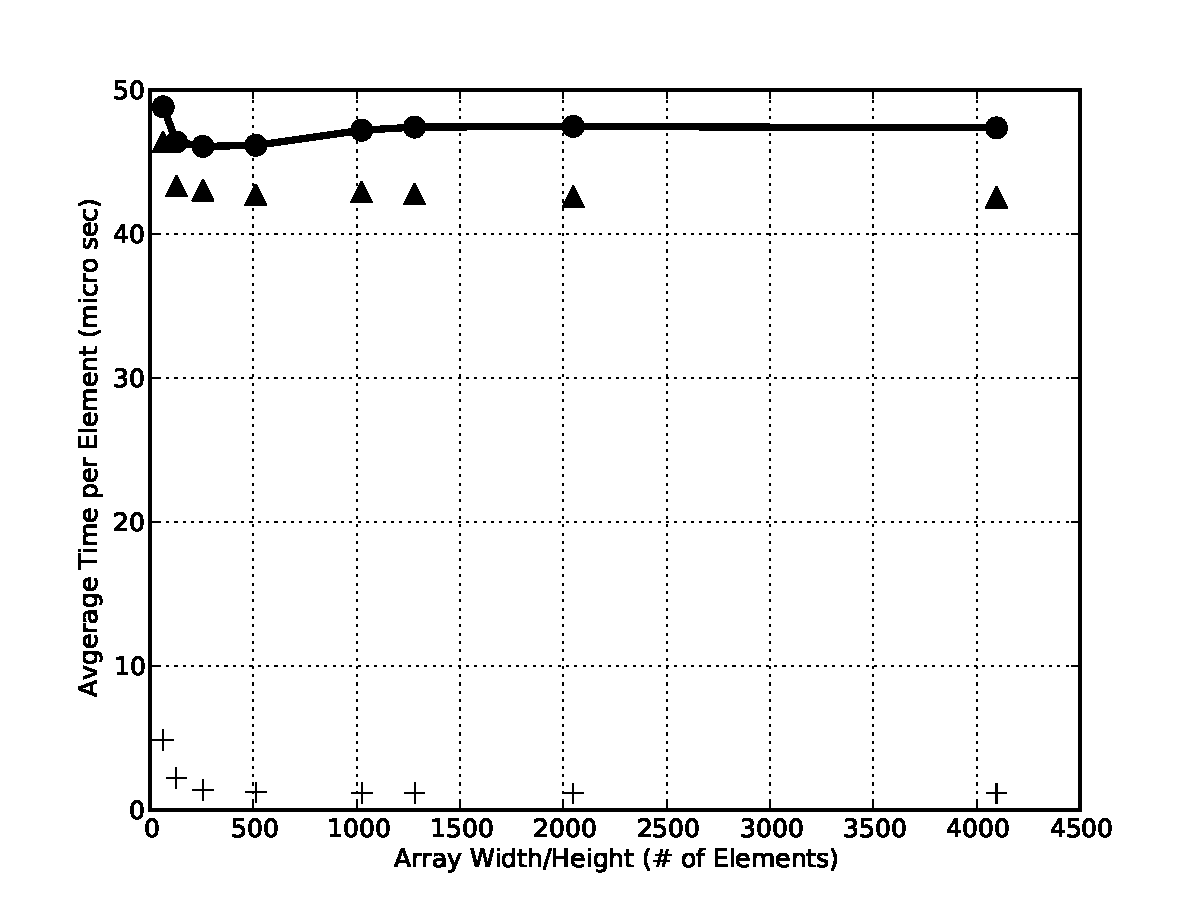
\includegraphics[width=2.5in]{cl-performance.pdf}
\caption{Performance comparison for varying array size.}
\label{fig:cl-performance}
\end{figure}
